
\section{Experiment and Result}

\subsection{Single-View Lip-Reading}
The table \ref{tab:singletb} shows results of various application of Bi-directional LSTM and Batch Normalization on single-view lip reading. 

\begin{table}[h]
\centering
    \begin{tabular}{c|cccccc}
        \multicolumn{1}{c|}{Accuracy(\%)} &%
        \multicolumn{6}{c}{Single-View}\\ \hline
        Model  &% BN &% Data-Aug &%
        Frontal & 30\si{\degree}& 45\si{\degree} & 60\si{\degree} & Profile & Avg\\\hline
        %
        BaseLine%
        &% LSTM &% \multirow{2}{*}{SVM} &%
        81.1& 80& 76.9& 69.2& 82.2&77.9\\
        %&% biLSTM &% &% & & & & &\\
        Bi-LSTM%
        &% LSTM &% \multirow{2}{*}{SVM} &%
        80.28& 75.28& 83.89& 75.83& 82.5&80.66\\
        %&% biLSTM &% &%
        %& & & & &\\
        BN%
        &% LSTM &% \multirow{2}{*}{SVM} &%
        80.56& 77.78& 78.61& 73.89& 72.78&76.72\\
        %&% biLSTM &% &%
        %& & & & &\\
        Bi-LSTM+BN%
        &% LSTM &% \multirow{2}{*}{SVM} &%
        84.72& 81.39& 82.78& 76.94& 81.1&81.39\\
        %&% biLSTM &% &%
        %& & & & &\\
    \end{tabular}
    \caption{Results on Single-view experiments. BN for Batch Normalization}
    \label{tab:singletb}
\end{table}

\subsubsection{Bi-directional LSTM}
\subsubsection{Batch Normalization}
Adding Batch Norm layer after LSTM was effective but not as Bi-LSTM. It	has incresed only for 45 and 60 degree of view. Besides, it even degregated the accuracy harshly on profile view. However, combination of Bi-LSTM and Batch Normalization boost the performance of overall view compare to only BN application and also compare to baseline except profile view. 	


\subsection{Multi-View Lip-Reading}
\subsubsection{Visual Model Architecture}
The table \ref{tab:multitb} shows similar application of Bi-directional LSTM and Batch Normalization on four different visual model. 
\begin{table}[h]
\centering
    \begin{tabular}{c|cccc}
        \multicolumn{1}{c|}{Accuracy(\%)} &%
        \multicolumn{4}{c}{Multi-View}\\ \hline
        Model&%  & BN & Data-Augment &%
        3D-CNN & MC & MI & MF \\\hline
        %
        BaseLine%\multirow{2}{*}{CNN+key}%
        & %LSTM% & \multirow{2}{*}{SVM} &%
        76.1 & 78.9& 80.0& 79.4\\
        %& %biLSTM %& &%
        % & & & &\\
        Bi-LSTM%\multirow{2}{*}{CNN+opti}%
        & %LSTM% & \multirow{2}{*}{SVM} &%
        76.94 & 79.17& 80.0& 81.11\\
        %& %biLSTM% & &%
        % & & & &\\
        BN%\multirow{2}{*}{Alex+key}%
        & %LSTM% & \multirow{2}{*}{SVM} &%
         82.78& 84.44& 81.94& 82.22\\
        %& %biLSTM% & &%
        % & & & &\\
        Bi-LSTM+BN%\multirow{2}{*}{Alex+opti}%
        & %LSTM% & \multirow{2}{*}{SVM} &%
         83.33& 87.22& 83.89& 88.06\\
        %& %biLSTM% & &%
        % & & & &\\
    \end{tabular}
    \caption{Results of Multi-View experiments. BN for Batch Normalization, MC for Merge Channels, MI for Merge Images and MF for Merge Feature.}
    \label{tab:multitb}
\end{table}


\subsubsection{Data-Augmentation}
We implemented data-augmentation as explained in method part, and the impact of data-augmentation explicitly proves its effectiveness, as it finally perform the best in three combination of bi-LSTM, Batch Normalization and data-augmentation.
\begin{table}[h]
	\centering
	\begin{tabular}{c|cccc}
		\multicolumn{1}{c|}{Accuracy(\%)} &%
		\multicolumn{4}{c}{Multi-View with Data Augmentation}\\ \hline
		Model&%  & BN & Data-Augment &%
		3D-CNN & MC & MI & MF \\\hline
		%
		Data-Augment%\multirow{2}{*}{CNN+key}%
		& %LSTM% & \multirow{2}{*}{SVM} &%
		77.29 & 79.36& 82.12& 81.25\\
		%& %biLSTM %& &%
		% & & & &\\
		Bi-LSTM%\multirow{2}{*}{CNN+opti}%
		& %LSTM% & \multirow{2}{*}{SVM} &%
		78.30 & 79.17& 80.0& 81.85\\
		%& %biLSTM% & &%
		% & & & &\\
		%BN%\multirow{2}{*}{Alex+key}%
		%& %LSTM% & \multirow{2}{*}{SVM} &%
		%82.78& 84.44& 81.94& 82.22\\
		%& %biLSTM% & &%
		% & & & &\\
		Bi-LSTM+BN%\multirow{2}{*}{Alex+opti}%
		& %LSTM% & \multirow{2}{*}{SVM} &%
		87.78& 88.89& \textbf{90.00}& 89.17\\
		%& %biLSTM% & &%
		% & & & &\\
	\end{tabular}
	\caption{Results of Multi-View experiments with Data Augmentation.}
	\label{tab:multitbaug}
\end{table}


\subsection{Confusion Matrix Results}
\begin{figure}[h]
	\centering
	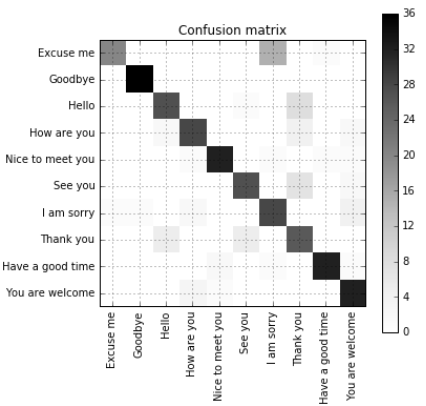
\includegraphics[width=0.48\columnwidth]{fig/multi80MI.png}
	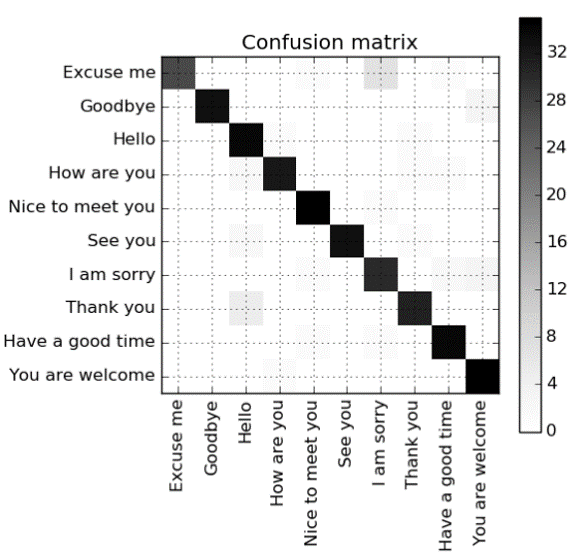
\includegraphics[width=0.5\columnwidth]{fig/multi90MI.png}
	\caption{Confusion Matrix of Merge Image architencture. The left image is for BaseLine(Accuracy of 80\%) and the right image is for Bi-LSTM+BN with Data Augmentation model(Accuracy of 90\%).  x-axis is predicted label and y-axis is true labels.}
	\label{fig:multi80MI}
\end{figure}
There is difference in accuracy of 10 percentage between baseline multi-view Merge Image visual model, and its extension of bi-directional LSTM, batch-normailzation and data augmentation. We can that difficulties on 'Excues me' had eased and the other confusions. However, there still have slight difficulties on 'Excuse me' to 'I am sorry' and 'Thank you' to 'Hello', which can be seen as confusion of pronouncation similaities.
%\begin{figure}[h]
%	\centering
%	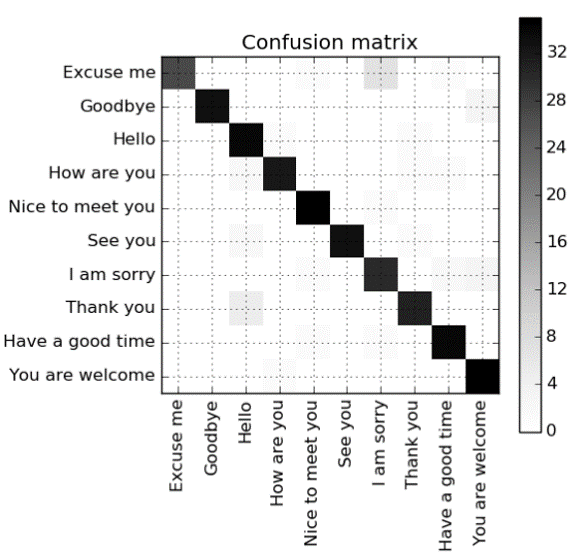
\includegraphics[width=0.5\columnwidth]{fig/multi90MI.png}
%	\caption{confusion Matrix of Merge Image architencture for Bi-LSTM+BN with Data Augmentation model. .}
%	\label{fig:multi90MI}
%\end{figure}


%
%\subsection{Single-view Lip-Reading}
%
%\begin{figure}[h]
%	\centering
%	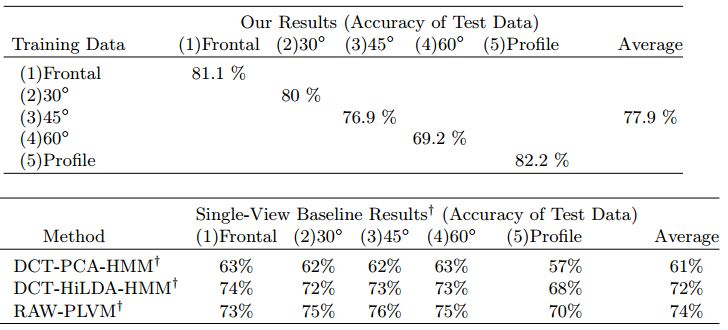
\includegraphics[width=\columnwidth]{fig/s1.jpg}
%	\caption{Single-view test accuray of word phrases.}
%	\label{fig:s1}
%\end{figure}
%Fig \ref{fig:s1} shows the accuracy result of single - view on word phrase test data. The results are similar to the one presented in \cite{Lee}. We have best accuracy on Profile view.
%
%\begin{figure}[h]
%	\centering
%	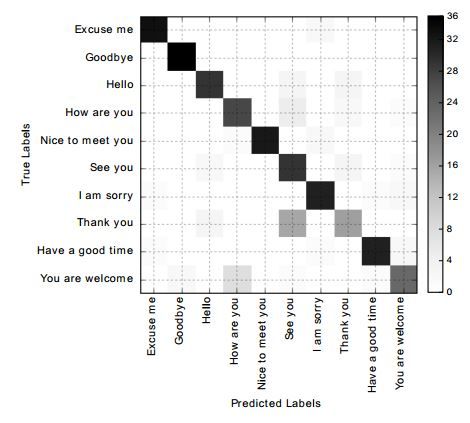
\includegraphics[width=\columnwidth]{fig/s2.jpg}
%	\caption{Confusion matrix of best of Single Views}
%	\label{fig:s2}
%\end{figure}
%Fig \ref{fig:s2} is Confusion matrix of profile view, which is the best in single view test accuracy. The x-axis is prediction classes and the y-axis is true classes.
%We can see that 'Thank you' and 'See you' is the most confusing word phrase.
%
%
%\subsection{Cross-view Lip-Reading}
%In Cross view experiment, we conduct it as two seperate stages. At first stage, as we refer it to 'Cross View(CV)', we train 5 total view data all together simultaneously and test each view seperately.  In this approach, we get the
%average accuracy 82.6\%, and all of the results are better than preliminary results.
% At Second stage, we call this stage as "Cross-view2(CV2)", and here, we finetune the first stage result to a certain view and also test with the certain view. Here, we can see slightly better performance on each view and also on average compare to CV.
%  
%\begin{figure}[h]
%	\centering
%	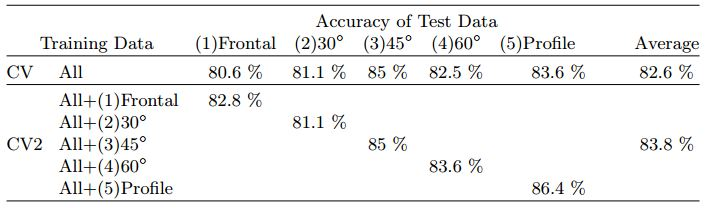
\includegraphics[width=\columnwidth]{fig/c1.jpg}
%	\caption{Cross-view test accuracy. CV : Cross View, CV2 : Cross View 2}
%	\label{fig:c1}
%\end{figure}
%In CV, Profile view shows the best performance(83.6\%), and in CV2, 60-degree view shows the best performance on total Cross view experiment.
%
%\begin{figure}[h]
%	\centering
%	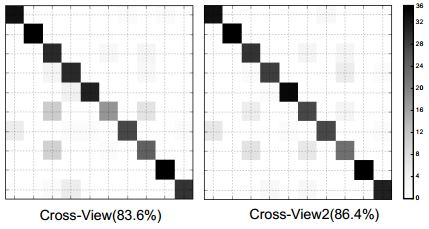
\includegraphics[width=\columnwidth]{fig/c2.jpg}
%	\caption{Confusion matrices of best of  Cross Views}
%	\label{fig:c2}
%\end{figure}
%The confusion matrices of test accuracies of profile view(CV) and 60-degree view (CV2). The axis lable share the same label in fig \ref{fig:s2}. It shows that
%a gradual improvement from single-view to cross-view.  
%
%\subsection{Multi-view Lip-Reading}
%In Multi-view experiment, we conduct slightly different type of architecture as inputs are five times larger then single or cross view experimetn. Here, we conduct Merge Image method as this method of multi-view is best in our previous paper.
%
%\subsubsection*{Merge Images}
%\begin{figure}[h]
%	\centering
%	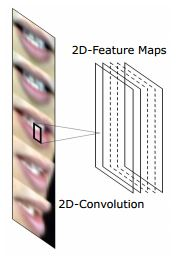
\includegraphics[width=0.4\columnwidth]{fig/mi.jpg}
%	\caption{Merge Image model architencture for the multi-view setting}
%	\label{fig:mi}
%\end{figure}
%As shown in fig \ref{fig:mi}, we append five images from the different
%view at the same time into a single image as an input of the visual model. In this
%architecture, we expect to learn all the five view feature by 2D-CNN. While out
%of our experiment, a more elaborate configuration is that all five images avoid
%convolving each other along the edges.
%
%Despite it has more feature (give times more inputs), the result is worse than cross-view.
%Fig \ref{fig:summary} shows the summary of all experiment through this paper.
%\begin{figure}[h]
%	\centering
%	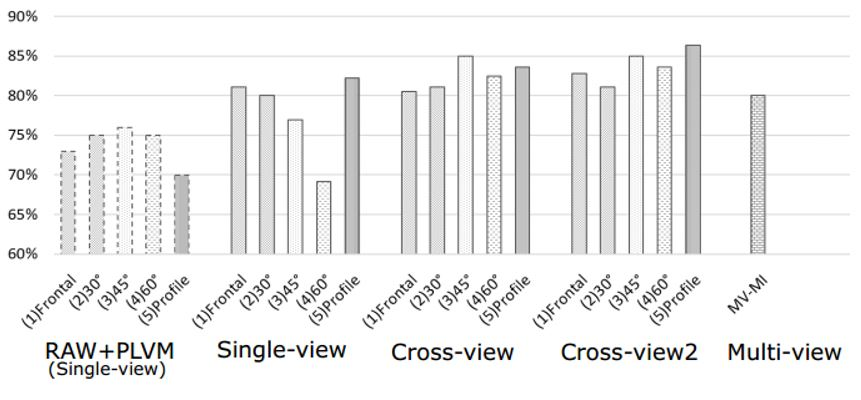
\includegraphics[width=\columnwidth]{fig/summary.jpg}
%	\caption{The summary of the accuraciese. MV-MI is refers to Merge Images.}
%	\label{fig:summary}
%\end{figure}
